\documentclass[11pt]{article}
\usepackage{amsmath,amssymb, amsthm, marvosym, permute, extsizes}
\usepackage{ graphicx, float, enumitem, adjustbox, hyperref, bm}
\usepackage[separate-uncertainty = true]{siunitx}
\usepackage{microtype, dsfont}
\usepackage[normalem]{ulem}
\usepackage{braket}
\usepackage[T1]{fontenc}
\usepackage[utf8]{inputenc}
\usepackage[justification=centering]{caption}
\usepackage{lmodern}
\usepackage{mhchem}
\usepackage{gensymb}
\usepackage[T1]{fontenc}
\usepackage[a4paper,margin=2.5cm]{geometry}
\usepackage[icelandic]{babel}
\usepackage{tikz}
\newcommand{\explain}[2]{\underbrace{#1}_\textrm{$#2$}}
\usepackage{minted}
\usemintedstyle{perldoc}
\parindent = 0pt
\usepackage{fancyhdr}
    \pagestyle{fancy}
    \headheight=32pt
    \lhead{Háskóli Íslands\\Raunvísindadeild}
    \rhead{Verkleg Eðlisfræði}
\title{{\Huge Segulvægi}}
\author{Emil Gauti Friðriksson \& Garðar Árni Skarphéðinsson}
\date{Apríl 2019 \\
\vspace{5cm}

\includegraphics[width = .6\textwidth]{HIlogo1.png}}

\begin{document}

\maketitle
\thispagestyle{empty}

\newpage

\section{Inngangur}
Í þessari tilraun var hegðun síseguls í ytra segulsviði skoðuð. Sú hegðun er síðan tengd við segulvægi hans, $\Vec{\mu}$, og gildi þess reiknað. Tilrauninni er skipt í fjóra hluta, eða raunar í fjórar mismunandi tilraunir, sem allar byggjast á sömu uppstillingu og hafa það sameinignlega markmið að finna styrk $\Vec{\mu}$.
\section{Uppstilling}
Uppspretta ytra segulsviðsins í þessari tilraun voru Helmholtz spólur með $195$ vafningum á hvorri spólu. Þegar straumur rennur um þannig spólu verður segulsviðið í miðju hennar nær alveg einsleitt, og þar var því komið fyrir járnseglinum sem skoða átti. Segulinn situr í miðjunni á hringlaga kúlu, en utan á þessari kúlu er stútur og hefur seglinum verið stillt upp þannig að stefna segulvægis hans sé samsíða þessum stút. Þessari kúlu er síðan komið fyrir á milli Helmholtz spólanna og látin sitja ofan á loftpúða sem búinn er til með loftdælu, svo að hún geti snúist nær viðnámslaust og fylgt segulvægi járnsegulsins. \\
Spólan er tengd við straumgjafa sem gerir okkur kleift að stjórna rafstraumnum sem rennur um hana, en einnig getum við kveikt á ljósi sem blikkar með tiltekinni tíðni og breytt áttun annarar spólunnar til þess að fá ósamleitið segulsvið. Þessir þættir koma til sögu síðar í tilrauninni. 

\begin{table}[H]
    \centering
        \caption{Lengdarmælingar.}
    \begin{tabular}{|l|c|c|}
    \hline
    Mælt var                &Algebraísk heiti   & Stærð \\
    \hline
    Radíus kúlu             &$R_K$              &$\SI{26.70\pm0.03}{mm}$\\
    Radíus Helmholts-spólu  &$R_H$              &$\SI{0.109}{m}$\\
    Lóðrétt bil á milli Helmholts-spóla&$h_H$   &$\SI{0.138}{m}$\\
    Fjöldi snúninga í Helmholts-spólu  & $N_H$  &$\SI{195}{}$\\
    Lengd stúts             &$L_s$              &$\SI{12.4\pm0.1}{mm}$\\
    \hline
    \end{tabular}

    \label{tab:lengdir}
\end{table}
\begin{table}[H]
\centering
    \caption{Massamælingar, Óvissa er hverfandi lítil.}
    \begin{tabular}{|l|c|c|}
    \hline
    Mælt var                &Algebraísk heiti   & Stærð \\
    \hline
    Massi lóðs(Hluti 1)     &$m_L$              &$\SI{1.3588}{g}$\\%Muna að segja að óvissa sé hverfandi
    Massi kúlu              &$M_K$              &$\SI{141.5868}{g}$\\
    Massi þyngri bolta/lóða &$M_b$              &$\SI{1.1267}{g}$\\
    Massi léttari bolta/lóða&$m_b$              &$\SI{0.4755}{g}$\\
    Massi lóðs(Hluti 4)     &$M_L$              &$\SI{137.9464}{g}$\\
    \hline
    \end{tabular}
    \label{tab:massar}
\end{table}

\section{Framkvæmd og úrvinnsla}
\subsection{Jafnvægi segulkrafts og þyngdarkrafts}
Í þessum hluta tilraunarinnar framlengjum við stút kúlunnar með stöng og lóði á stönginni. Stöngin og lóðið gefur kúlunni kraftvægi vegna þyngdarkrafts þegar stúturinn myndar horn við hið lóðrétta. 

\begin{figure}[H]
  \centering
    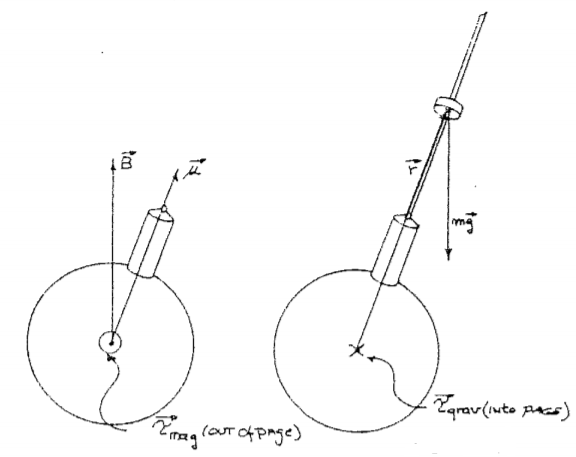
\includegraphics[width=130mm]{g_torque.PNG}
    \caption{Stöng með lóði komið fyrir í stútnum á kúlunni. Þyngdarkraftur verkar á lóðið og veldur kraftvægi.}
    \label{fig:g_torque} 
\end{figure}

Kraftvægið sem kúlan fær vegna þyngdarkraftsins sem verkar á lóðið er $\tau_g = \Vec{r} \times m_L\Vec{g}$, þar sem $\Vec{g}$ er þyngdarhröðun jarðar og $r = R_K + L_s + x$ er fjarlægðin frá miðju kúlunnar að lóðinu. Hér er $x$ mæld fjarlægð frá brún stútsins að miðju lóðs. Ef sett er á segulsvið $\Vec{B}= B \Hat{z}$ þá fæst þó einnig kraftvægi vegna segulkrafta, þ.e. $\tau_m =\Vec{\mu} \times \Vec{B}$. \\
Við aukum strauminn sem rennur um spólurnar, og þar með styrk segulsviðsins, þangað til að stöngin með lóðinu byrjar að lyftast og liggur samsíða hinu lárétta. Þetta gerist þegar kraftvægin vegna þyngdar- og segulkraftsins eru í jafnvægi, það er að segja þegar
\begin{equation}
\Vec{r} \times m_L\Vec{g} = \Vec{\mu} \times \Vec{B}.  \label{eq:jafnvaegis}  
\end{equation}
Þetta gerist fyrir ákveðið straumgildi, en út frá því gildi má síðan reikna styrk segulsviðsins, sem þá má stinga í jafnvægisjöfnuna~(\ref{eq:jafnvaegis}) til þess að reikna segulvægi járnsegulsins. \\
Stöðu lóðsins á stönginni, $x$, var breytt nokkrum sinnum og fyrir hverja stöðu var straumurinn sem þurfti til þess að fá vægisjafnvægi fundinn. Við þetta jafnvægi gildir

\begin{align}
r = \frac{\mu}{m_L g}B
\end{align}

Við setjum því mælingarnar okkar upp sem graf af $B$ á móti $r$, og hallatala bestu línu ætti þá að vera $\mu/m_L g$.

\begin{figure}[H]
    \centering
    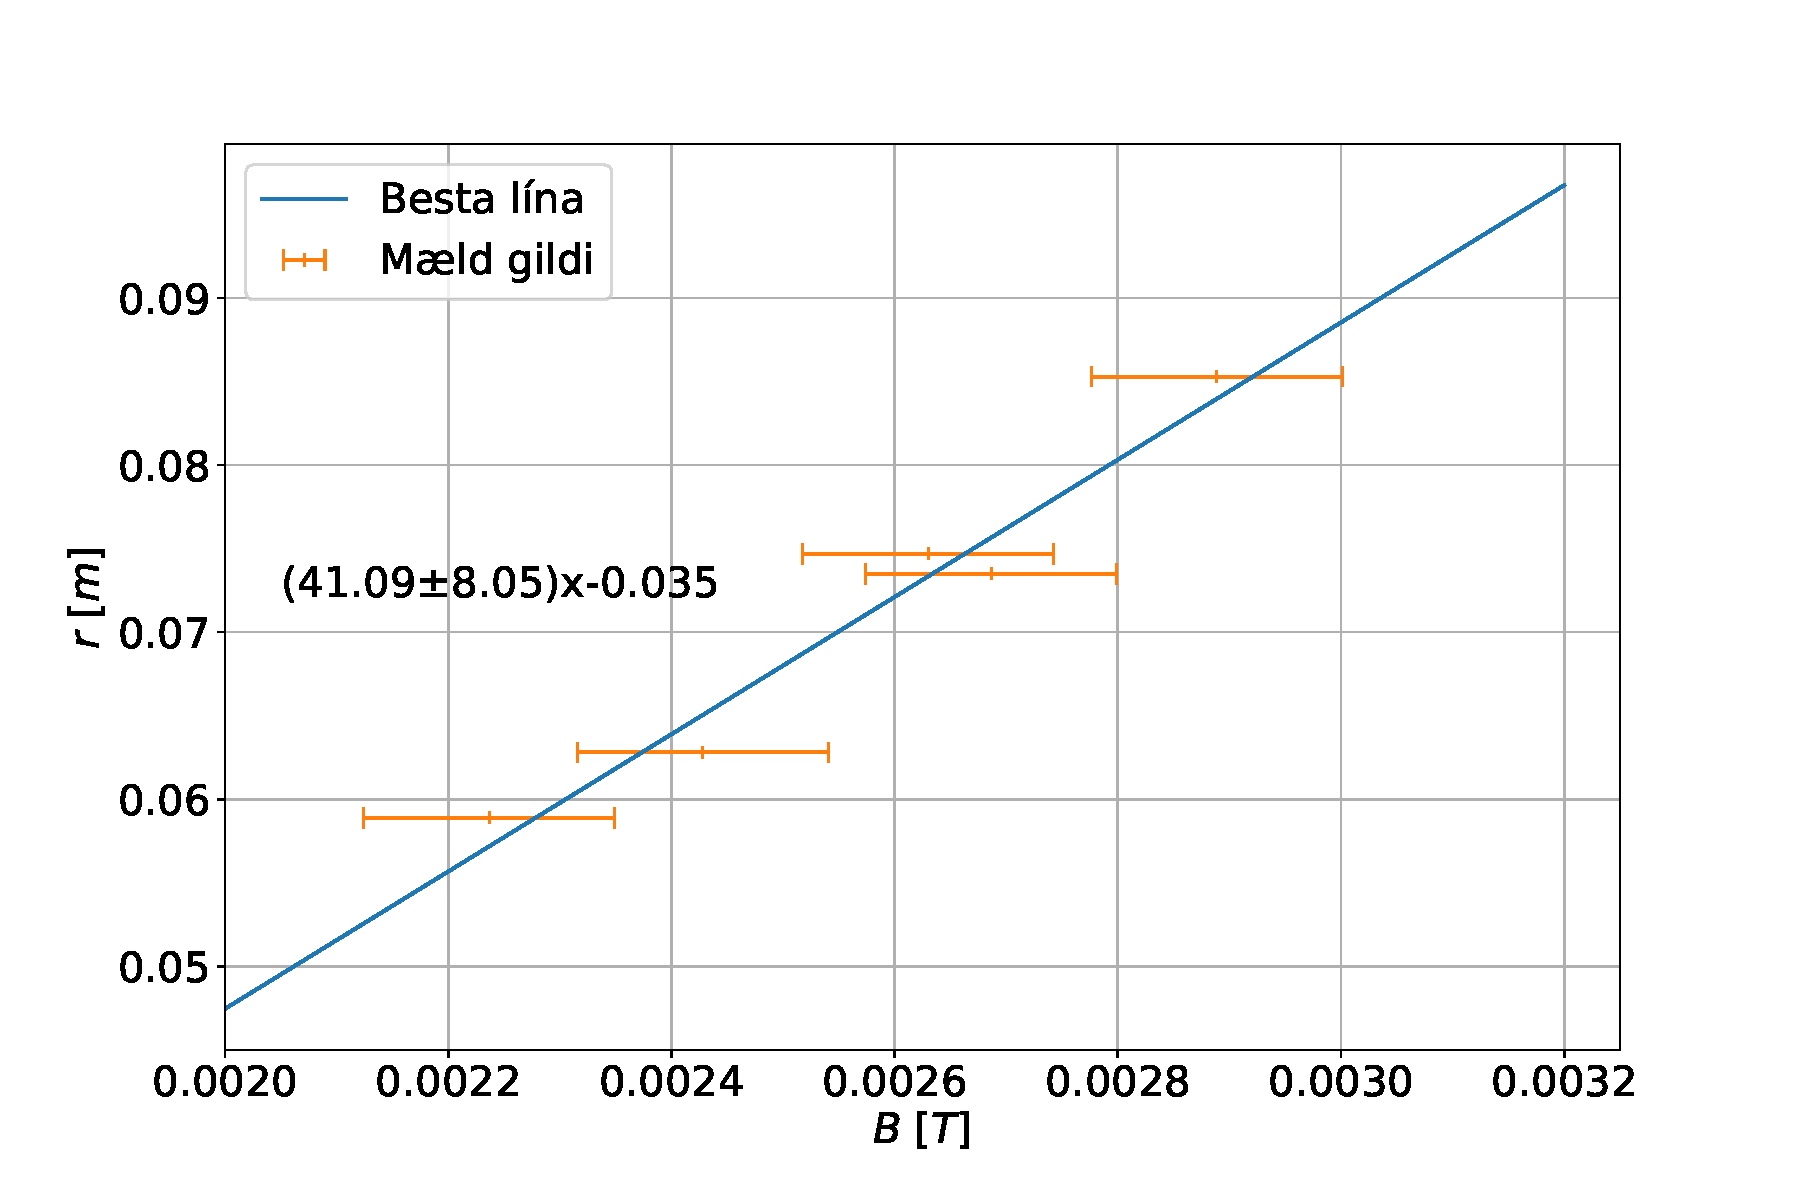
\includegraphics[width=0.7\textwidth]{Hluti_1.PDF}
    \caption{Fjarlægð lóðs frá miðju kúlu sem fall af styrk ytra segulsviðs. Hallatala bestu línu er $41.09 \pm 8.05$, en það gefur segulvægið $\mu_1 = \SI{0.548 \pm 0.107}{A m^2}$.}
    \label{fig:hluti 1}
\end{figure}

\subsection{Hreintóna sveifla}
Í þessum hluta tilraunarinnar voru stöngin og lóðið fjarlægð þannig að allt þyngdarkraftvægi væri hverfandi. Kúlunni var komið fyrir í segulsviði þannig að segulvægið beindi beint upp. Síðan var ýtt við stútnum á kúlunni þannig að lítið horn $\theta$ myndaðist á milli stefnu ytra segulsviðsins og segulvægis kúlunnar. Segulkraftvægið leitast þá við að rétta þessa hliðrun af og kúlan byrjar að vagga fram og til baka. Þessari hreintóna sveiflu má lýsa með afleiðujöfnunni 

\begin{align}
|-\Vec{\mu} \times \Vec{B}| = -\mu B \sin(\theta) = I \frac{d^2 \theta}{dt^2}
\end{align}

Þar sem $I = \frac{2}{5}M_K R_K^2$ er hverfitregða kúlunnar. Þar sem hornið $\theta$ er lítið getum við notað nálgunina $\sin(\theta) \simeq \theta$ og fengið

\begin{align}
-\mu B \theta = I\frac{d^2\theta}{dt^2}
\end{align}

Við gerum ráð fyrir lausn á þessari hornbreytingu í tíma á forminu $\theta(t) = A\cos(\omega t)$ fyrir eitthvað fast útslag $A$ og horntíðni $\omega$. Fyrir þessa lausn verður afleiðujafnan að ofan að

\begin{align}
-\mu B A\cos(\omega t) = -I\omega^2 A \cos(\omega t)
\end{align}

En þetta leiðir af sér jöfnuna

\begin{align}
\omega^2 = \left( \frac{2\pi}{T} \right)^2 = \frac{\mu B}{I}
\end{align}

Þar sem $T$ er sveiflutími kúlunnar. Um sveiflutímann gildir þá að 

\begin{align}
T^2 = \frac{4\pi^2 I}{\mu B}
\end{align}

og þetta samband getum við notað til þess að finna segulvægið $\mu$. Við komum af stað sveiflu og mælum sveiflutímann $T$. Til þess að fá nákvæmara gildi á hana mælum við tímann sem það tekur okkur að fá tíu sveiflur, $T_{10}$, og látum svo $T = T_{10}/10$. Þessi mæling er síðan framkvæmd fyrir mismunandi gildi á $B$ og sett er upp graf af $T^2$ á móti $1/B$. Hallatala bestu línu þessa grafs ætti þá að vera $4\pi^2I/\mu$.

\begin{figure}[H]
    \centering
    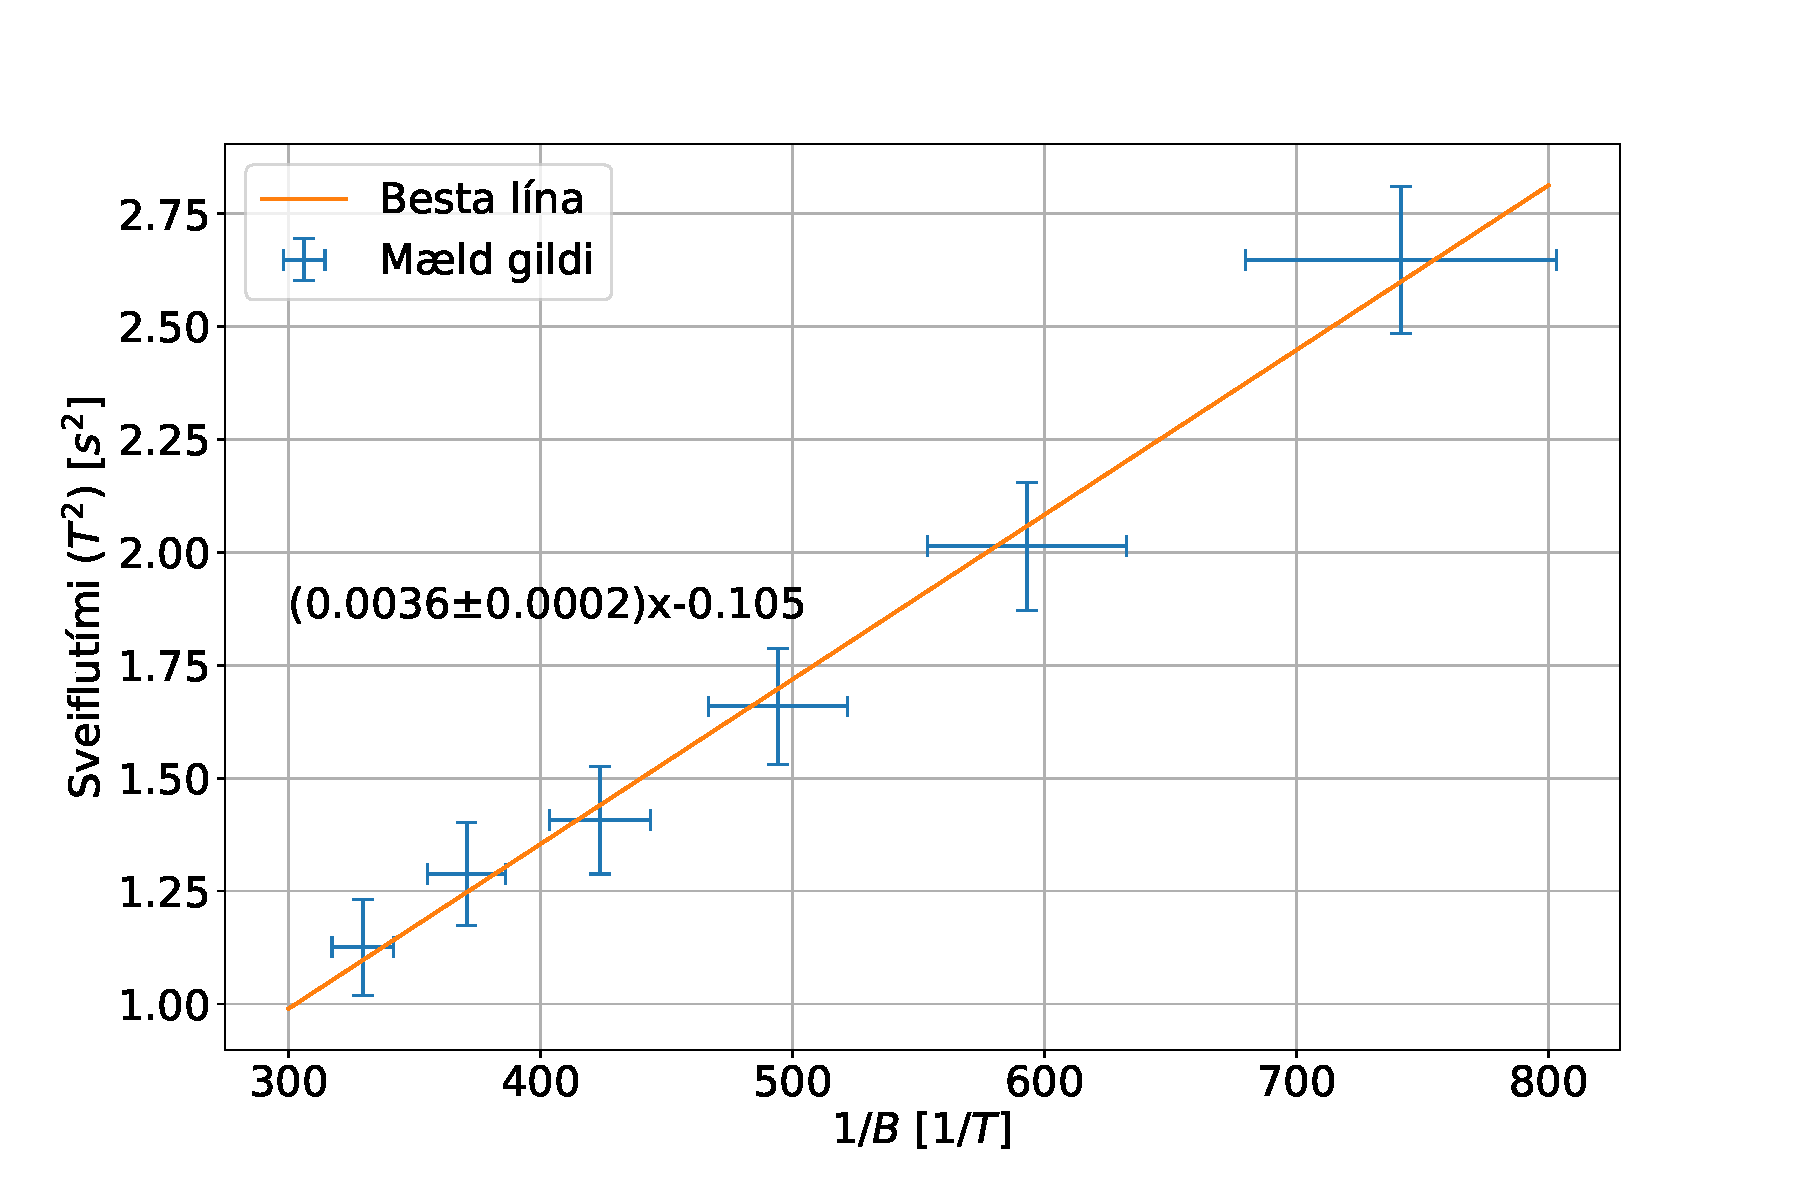
\includegraphics[width=0.7\textwidth]{Hluti_2.PDF}
    \caption{Sveiflutími í öðru veldi sem fall af $1/B$. Hallatala bestu línu er $0.0036 \pm 0.0002$, en það gefur segulvægið $\mu_2 = \SI{0.437 \pm 0.039}{A m^2}$.}
    \label{fig:hluti 2}
\end{figure}

\subsection{Pólvelta}
Í þessum þriðja hluta tilraunarinnar er segulsvið Helmholtz spólanna notað til þess að koma af stað pólveltu á kúlunni. Við byrjum með ekkert segulsvið og stillum kúlunni upp á milli spólanna eins og áður. Við stillum henni upp þannig að stúturinn myndi horn $\theta '$ við hið lóðrétta og vefjum síðan löngu snæri utan um hann. Snærið er síðan togað af, en þá byrjar kúlan að snúast hratt um snúningsás sem er samsíða stefnu stútsins, það er að segja samsíða $\Vec{\mu}$. \\
Nú kemur blikkandi ljósið sem minnst var á hér áður til sögunnar. Ofan á stútnum er lítill hvítur blettur sem glampar þegar á hann skín ljós. Við kveikjum á ljósinu og fylgjumst bæði með þessum bletti sem blikkar í takt við ljósið, og uppgefinni tíðni ljóssins sem við lesum af straumgjafanum. Í fyrstu virðist manni eins og ljósi bletturinn á stútnum snúst mjög hratt samferða kúlunni, en ef að tíðni blikkandi ljóssins er breytt eða beðið er eftir því að snúningur kúlunnar hægist virðist þessi færsla punktsins einnig hægjast þangað til hann virðist loks standa í stað. Þegar punkturinn virðist alveg kyrr þýðir það að horntíðni kúlunnar er orðin jöfn blikktíðni ljóssins. Horntíðni kúlunnar fellur veldislega í tíma þannig að þegar hún hefur náð nógu lágu gildi má segja að hún verði nokkuð stöðug, og var sú tíðni valin sem $\SI{7.0}{Hz}$ hér. \\
Þegar þessari snúningstíðni er náð kveikjum við aftur á segulsviðinu. Við þetta fæst segulkraftvægi sem tengja má við breytingu hverfiþunga kúlunnar með jöfnunni

\begin{align}
\Vec{\mu} \times \Vec{B} = \frac{d\Vec{L}}{dt}
\end{align}

Hér er $\Vec{L} = \Vec{\omega}_s I$ hverfiþungi kúlunnar, en $\Vec{\omega}_s$ er hornhraði hennar. Þessi breyting á hverfiþunganum felst í því að eftir að segulsviðið er sett á heldur kúlan áfram að snúast um ás samsíða stútnum, en byrjar einnig að snúast um ás samsíða segulsviðinu. Við fáum semsagt pólveltu segulvægisins um stefnu segulsviðsins. Þessari pólveltu má lýsa með afleiðujöfnunni

\begin{align}
\frac{dL}{dt} = \Omega L \sin(\theta ')
\end{align}

Þar sem $\Omega$ er hornhraði pólveltunnar. Við fáum því

\begin{align}
|\Vec{\mu} \times \Vec{B}| = \mu B \sin(\theta ') = \Omega L \sin(\theta ')
\end{align}

Sem gefur okkur þá að $\Omega = \mu B/L$. \\
Við framkvæmum nú nokkrar mælingar. Í hvert skipti fáum við kúluna til að snúast um ás segulvægisins og bíðum þar til sú snúningstíðni nær um $\SI{7}{Hz}$, en þá kveikjum við á segulsviðinu. Fyrir mismunandi styrk á segulsviðinu mælum við tímann sem það tekur kúluna að snúast einn hring um ás segulsviðsins, $T_s$, og fáum út frá honum hornhraðann $\Omega = 2\pi/T_s$. Við setjum síðan upp graf af $\Omega$ á móti $B$ og ættum þá að fá bestu línu með hallatölu $\mu/L$.


\begin{figure}[H]
    \centering
    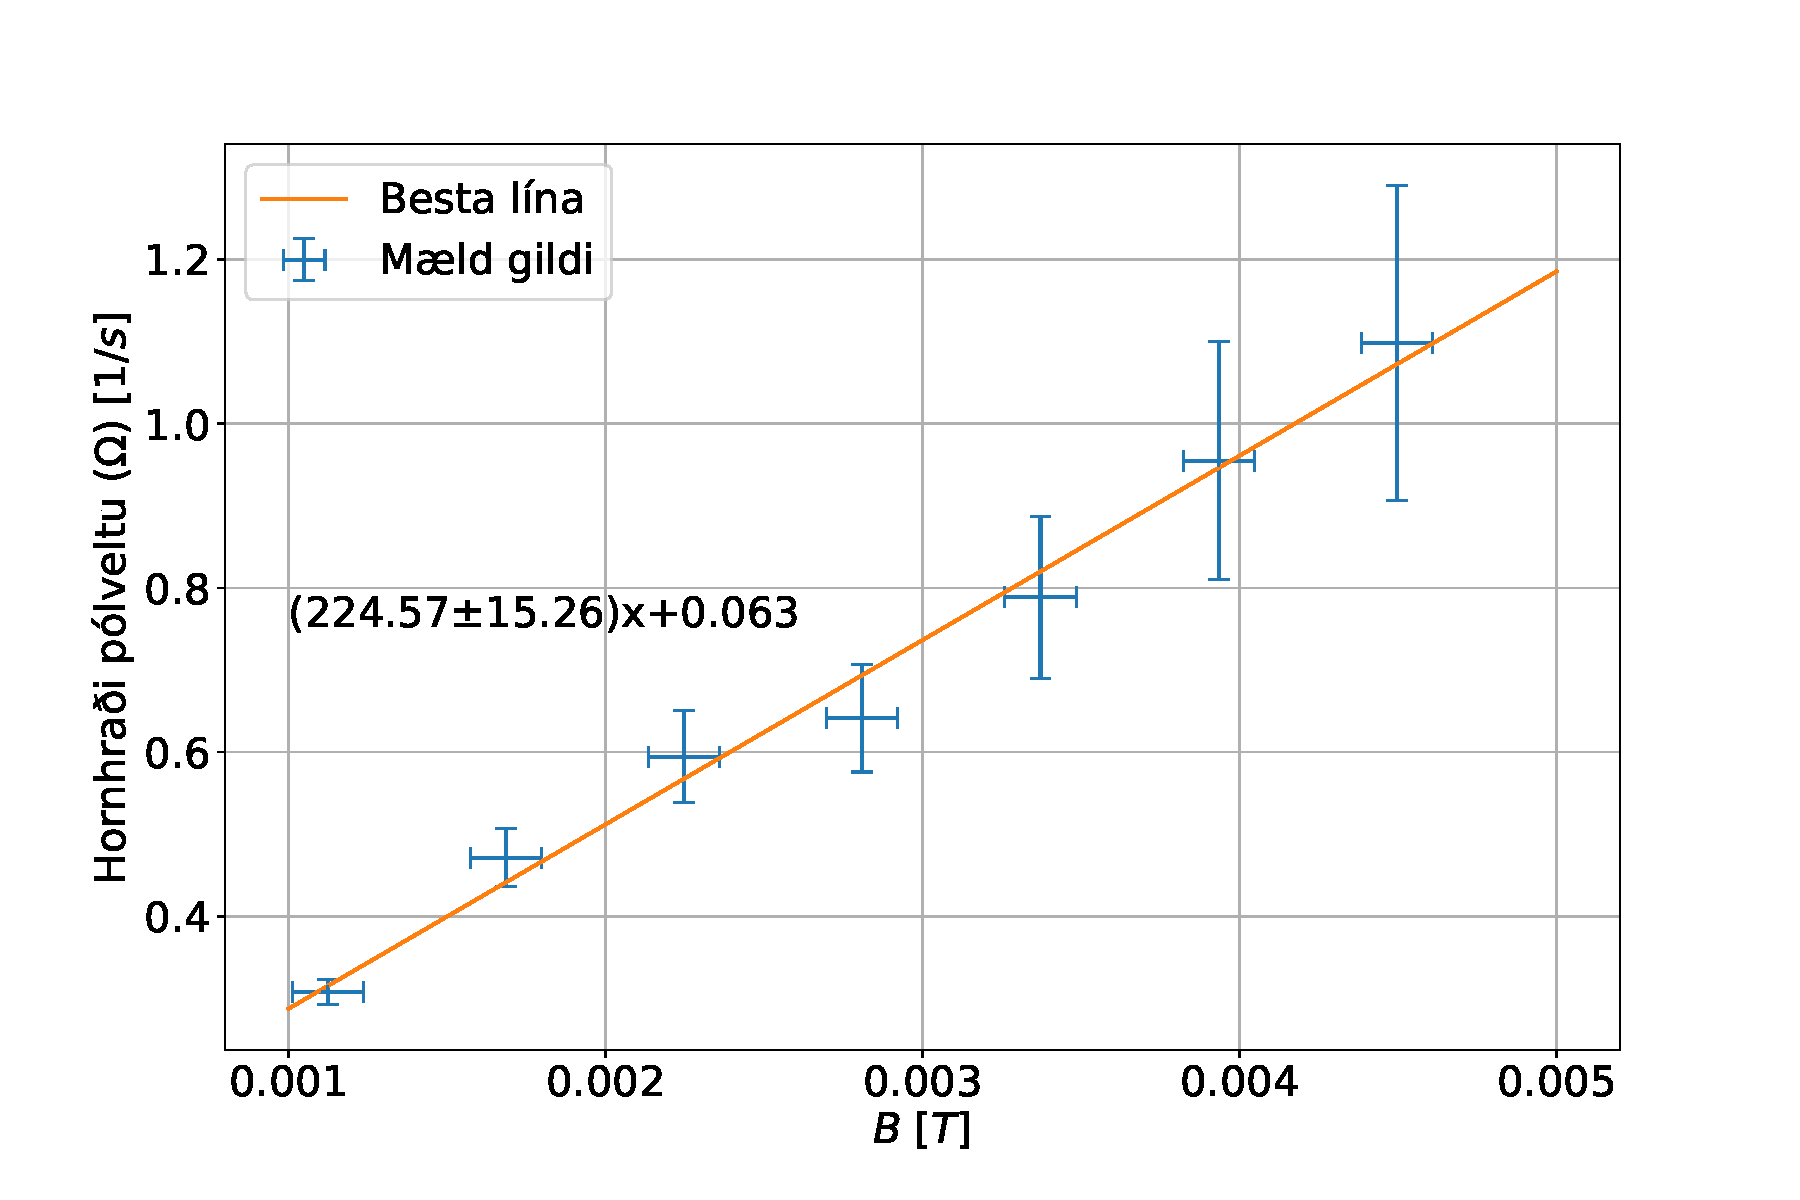
\includegraphics[width=0.7\textwidth]{Hluti_3.PDF}
    \caption{Hornhraði pólveltu sem fall af styrk segulsviðs. Hallatala bestu línu er $224.57 \pm 15.26$, en það gefur segulvægið $\mu_3 = \SI{0.399 \pm 0.028}{A m^2}$.}
    \label{fig:hluti 3}
\end{figure}

\subsection{Kraftur í óeinsleitu segulsviði}
Í þessum síðasta hluta tilraunarinnar stillum við Helmholtz spólurnar þannig að þær séu mismunandi áttaðar og spanni þar með segulsvið í gagnstæðar stefnur við hvora aðra. Í þessu tilfelli verður segulsviðið á milli þeirra ekki lengur einsleitt, heldur breytist það með hæð, og veldur þetta krafti í $\Hat{z}$-stefnu á járnsegulinn okkar sem situr í miðjunni. Þennan segulkraft má reikna með jöfnunni

\begin{align}
\Vec{F} = F\Hat{z} = \mu \frac{dB}{dz}\Hat{z}
\end{align}

Ef að þessi kraftur væri nógu mikill til þess að kúlan myndi byrja að lyftast upp þá gætum við borið hann saman við þyngdarkraftinn sem verkar á kúluna og þannig reiknað segulvægið. Því miður er kúlan of þung til þess. Við getum hins vegar fest band efst við stútinn á kúlunni, en þetta band liggur síðan á trissu og hinn endi þess að tengdur við lóð. Þá verður þyngdarkrafturinn sem verkar á kúluna $F_g = g(M_K - M_L)$. Lóðið er þannig að hægt er að bæta á það litlum málmkúlum til þess að þyngja það.\\
Við getum þá sett ákveðna þyngd á lóðið og síðan hækkað styrk segulsviðsins, og þar með $\frac{dB}{dz}$, og fundið hvað það þarf að vera hátt til þess að $F_g = \mu \frac{dB}{dz}$ og kúlan byrji að lyftast. Athugum einnig að $\frac{dB}{dz}$ er háð straumnum sem við setjum á spólurnar, $i$, þannig að

\begin{align}
\frac{dB}{dz} = (1.69 \cdot 10^{-2})i
\end{align}

Við endum þá með jafnvægisjöfnuna 

\begin{align}
g(M_K - M_{L+}) = \mu \frac{dB}{dz}
\end{align}
 
 Þar sem $M_{L+}$ er summa massa lóðsins og málmkúlanna. Ef við teiknum nú graf af $\frac{dB}{dz}$ á móti $M_{L+}$ þá ættum við að fá bestu línu með hallatölu $-g/\mu$.
 
\begin{figure}[H]
    \centering
    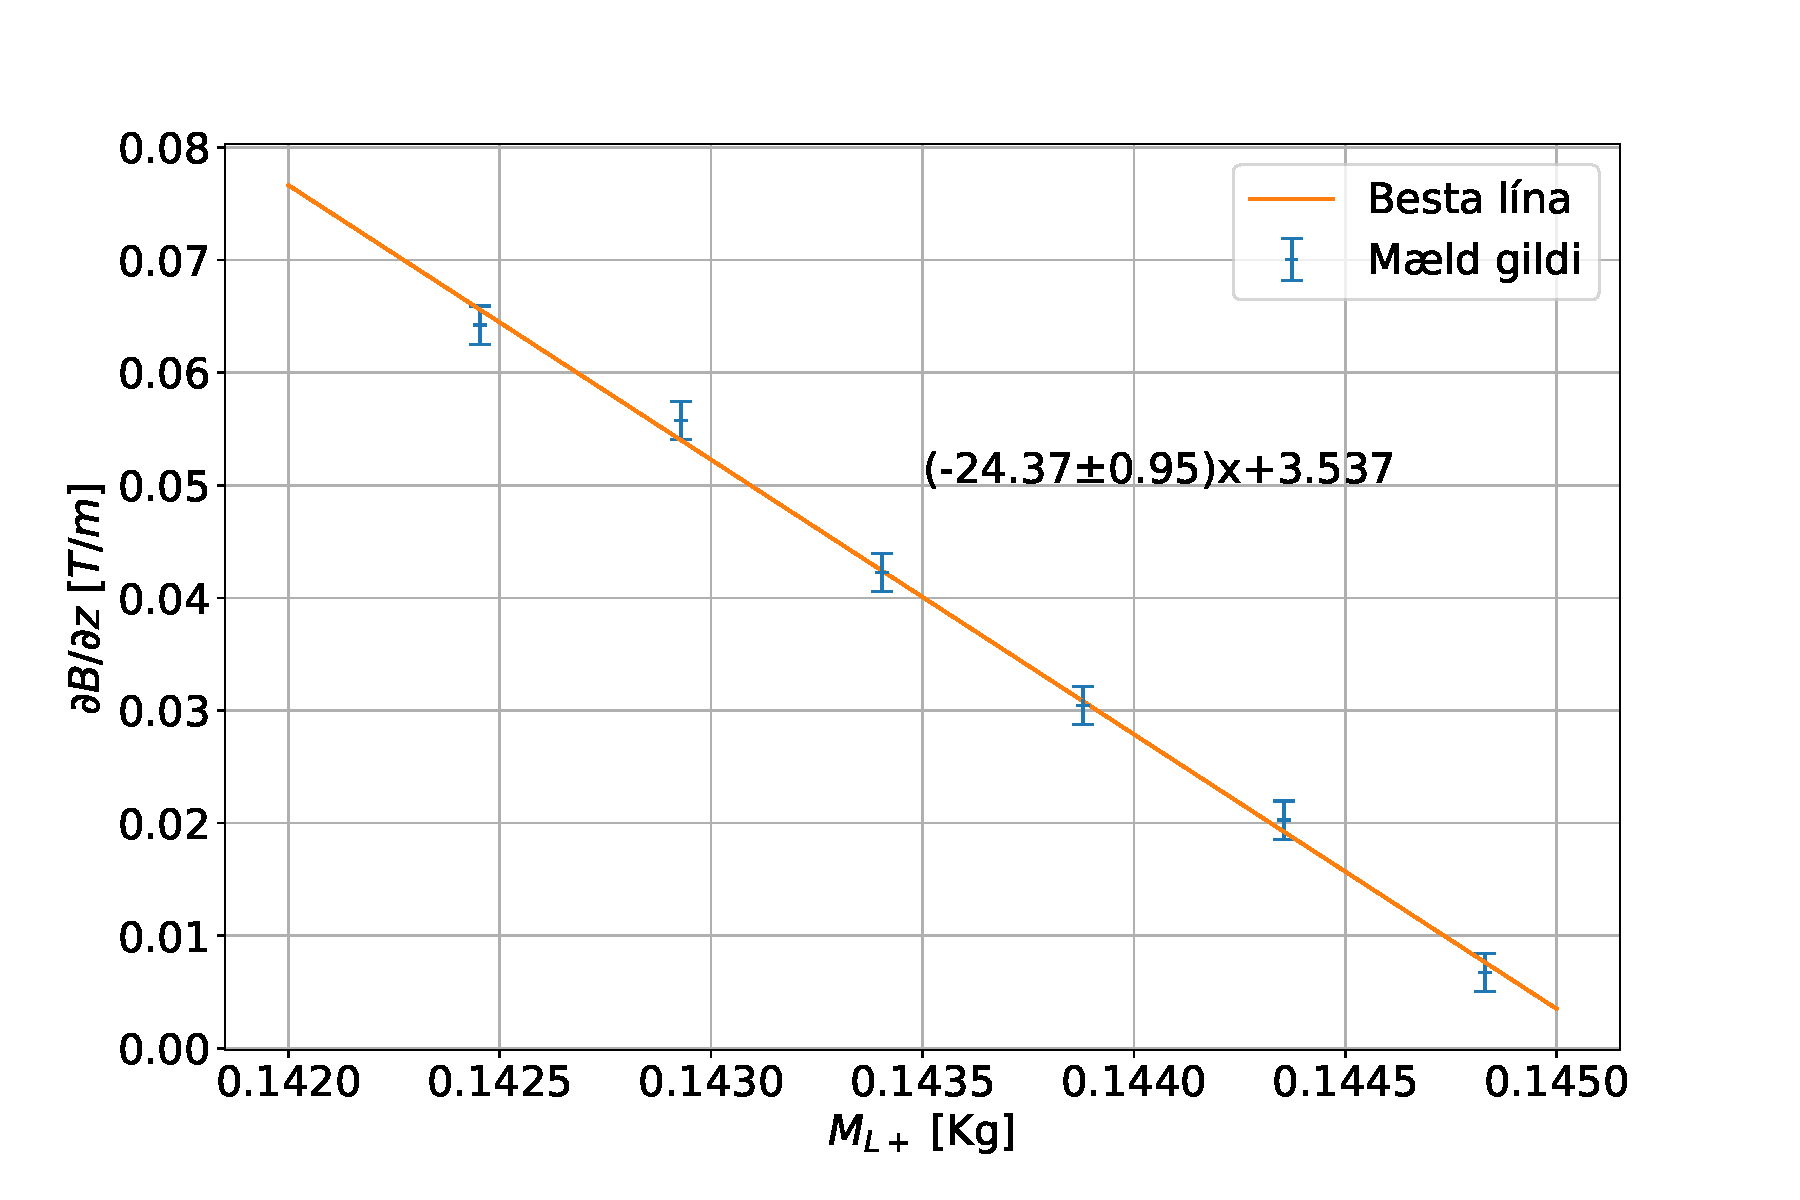
\includegraphics[width=0.7\textwidth]{Hluti_4.PDF}
    \caption{Stigull segulsviðs sem lyftir kúlunni sem fall af M_{L+}. Hallatala bestu línu er $-24.37 \pm 0.95$, en það gefur segulvægið $\mu_4 = \SI{0.403 \pm 0.016}{A m^2}$.}
    \label{fig:hluti 4}
\end{figure}
 
 
 
\section{Niðurstöður}

Í töflu~\ref{tab:samanburdur} sjást fjögur mismunandi gildin sem fengust fyrir segulvægi járnsegulsins og óvissur þeirra. Af þessu sést að gildin falla flest innan óvissumarka hvers annars og verður þessi tilraun því að teljast nokkuð vel heppnuð. Gildið $\mu_1$ liggur tiltölulega langt frá hinum þremur en hefur líka um það bil $20\%$ óvissu. Þessa ónákvæmni má útskýra með fljótfærni framkvæmenda og fjölda óvissuþátta.

\begin{table}[H]
    \centering
    \caption{Reiknuðu gildin fjögur á segulvæginu.}
    \begin{tabular}{|c|c|}
    \hline
    $\mu_i$     & Gildi\\
    \hline
    $\mu_1$     & $\SI{0.548 \pm 0.107}{A m^2}$  \\
    $\mu_2$     & $\SI{0.437 \pm 0.039}{A m^2}$  \\
    $\mu_3$     & $\SI{0.399 \pm 0.028}{A m^2}$ \\
    $\mu_4$     & $\SI{0.403 \pm 0.016}{A m^2}$  \\
    \hline
    \end{tabular}
    \label{tab:samanburdur}
\end{table}

\end{document}
